\let\mymarginpar\marginpar

\documentclass[10pt,twoside]{article}

%\long\def\authornote#1{%
%        \leavevmode\unskip\raisebox{-3.5pt}{\rlap{$\scriptstyle\diamond$}}%
%        \marginpar{\raggedright\hbadness=10000
%        \def\baselinestretch{0.8}\tiny
%        \it #1\par}}
%\newcommand{\ville}[1]{\authornote{NOTE TO SELF: #1}}

\usepackage{enumerate}% http://ctan.org/pkg/enumerate
%\usepackage{times}
\usepackage{amsmath,amsthm,amssymb}
\usepackage{fancyhdr}
\usepackage{moreverb}
\usepackage{graphicx}
\usepackage{amssymb}
\usepackage{url}
\usepackage{multirow} 
\usepackage[boxed, section]{algorithm}
%\usepackage{algorithm}
\usepackage{algorithmic}
%\usepackage{cite}
\usepackage{multirow} 
\usepackage{rotating}
\usepackage{geometry}
\usepackage{fix-cm}
\usepackage{subfigure}
\usepackage{natbib}
\usepackage{titlesec}
\usepackage{lipsum}
\usepackage{xstring}

\marginparwidth=1cm
\marginparsep=5pt
\newcommand\ville[1]{%
    \mymarginpar{\raggedright\hbadness=10000\tiny\it #1\par}}



\renewcommand{\baselinestretch}{1.2}
\setlength{\topmargin}{-0.7in}
\setlength{\textwidth}{6.2in}
\setlength{\textheight}{9in}
\setlength{\oddsidemargin}{0.2in}
\setlength{\evensidemargin}{0.2in}
\raggedbottom




\allowdisplaybreaks

\newcommand{\COR}{\text{COR}}
\newcommand{\POS}{\text{POS}}
\newcommand{\UNIT}{\text{UNIT}}
\newcommand{\LIN}{\text{LIN}}
\newcommand{\SD}{\text{SD}}

\newcommand{\myN}{\hbox{N\hspace*{-.9em}I\hspace*{.4em}}}
\newcommand{\myZ}{\hbox{Z}^+}
\newcommand{\myR}{\hbox{R}}
\newcommand{\R}{\mathbb{R}}
\newcommand{\PP}{{\bf P}}
\newcommand{\bLambda}{\boldsymbol{\lambda}}

\renewcommand{\P}{\mathbb{P}}
\newcommand{\E}{\mathbb{E}}
\newtheorem{defi}{Definition}
\newtheorem{theorem}{Theorem}[section]
\newtheorem{lemma}[theorem]{Observation}
\newtheorem{proposition}[theorem]{Proposition}
\newtheorem{observation}[theorem]{Observation}
\DeclareMathOperator*{\argmax}{arg\,max}
\DeclareMathOperator*{\argmin}{arg\,min}

\theoremstyle{definition}
\newtheorem{example}[theorem]{Example}

\theoremstyle{definition}
\newtheorem{definition}[theorem]{Definition}

\renewcommand{\abstractname}{}
\def\pb{\overline{p}}
\def\pt{\tilde{p}}
\def\one{{\bf 1}}

\def\bSigma{{\bf \Sigma}}
\def\bLambda{{\bf \Lambda}}
\def\blambda{\boldsymbol{\lambda}}
\def\bOmega{{\bf \Omega}}

\def\dd{{\bf d}}
\def\D{{\bf D}}
\def\v{{\bf v}}
\def\V{{\bf V}}
\def\s{{\bf s}}
\def\m{{\bf m}}
\def\r{{\bf r}}
\def\a{{\bf a}}
\def\e{{\bf e}}
\def\x{{\bf x}}
\def\q{{\bf q}}
\def\w{{\bf w}}
\def\A{{\bf A}}
\def\M{{\bf M}}
\def\X{{\bf X}}
\def\Q{{\bf Q}}
\def\L{{\bf L}}
%\def\R{{\bf R}}
\def\Z{{\bf Z}}
\def\B{{\bf B}}
\def\SS{{\bf S}}
\def\I{{\bf I}}
\def\F{{\cal F}}
\def\G{{\cal G}}
%\def\L{{\cal L}}
\def\P{{\mathbb P}}
\def\E{{\mathbb E}}
\def\Var{{\rm Var}\,}
\def\Cov{{\rm Cov}\,}
\def\Corr{{\rm Corr}\,}
\def\ee{\varepsilon}
\def\|{\, | \,}
\def\probit{p_{\rm probit}}
\def\plog{p_{\rm log}}
\def\conv{\text{conv}}
\def\cond{\text{cond}}
\def\diag{\text{diag}}
\def\vech{\text{vech}}
\def\vec{\text{vec}}
\def\Diag{\text{Diag}}
\def\diag{\text{diag}}
\def\Tr{\text{tr}}

\def\logit{{\rm logit}}

\newcommand{\myzrfunction}[1]
{\myfunction{#1}{{\myZ}}{{\myR}}}

\newcommand{\mysection}[1]
{\noindent {\bf {#1}}}
\begin{document}

%\title{Career Planning}
%\author{by\\
%\\
%Ville A. Satop\"a\"a\\
%\\
% \small Department of Statistics\\
% \small The Wharton School of the University of Pennsylvania\\
% \small Philadelphia, PA 19104- 6340, USA\\ [-0.25in]} \date{}
%%\small Center for Theoretical Physics\\
%%\small MIT 6-311, 77 Massachusetts Ave.\\
%%\small Cambridge, MA 02139-4307\\[-0.25in]} \date{} %% You could use \date{\small\today\today} to keep track
%%% of preliminary versions
%\maketitle


\titleformat{\section}
  {\normalfont\scshape}{\thesection}{1em}{}
\titleformat{\subsection}
  {\normalfont\scshape}{\thesubsection}{1em}{}


%\pagestyle{myheadings}
%\markboth{Ville A. Satop\"a\"a}{Research Statement}
\thispagestyle{empty}

\begin{center}
\Large
{\bf RESEARCH STATEMENT}\\
\normalsize
VILLE A. SATOP\"A\"A\\
THE WHARTON SCHOOL OF THE UNIVERSITY OF PENNSYLVANIA
%Ville A. Satop\"a\"a\\
%The Wharton School of the University of Pennsylvania
\end{center}
%\section*{Research Statement}

%Explain that i have two projects etc. To do justice to the time spent both should be described. Both are collaborative/inter disciplinary which I have enjoyed very much. 
%\section{Introduction}
%\vspace{-0.2em}
%In general I consider myself an applied statistician who enjoys cross-disciplinary collaboration and research problems with strong motivation in  interesting and relevant real-world data. 
\noindent
{\bf 1. INTRODUCTION:} For the past three years I have worked on two research projects that are not only topically very different but also have disjoint sets of collaborators. Both projects are highly interdisciplinary, involve much collaboration with subject-matter experts, and investigate research problems with strong motivation in  interesting and relevant real-world data. These projects are described in the following sections, starting with my dissertation work.


% \vspace{-0.2em}
%\section{Modeling, Aggregating, and Improving Predictions}  \vspace{-0.2em}
%\subsection*{Motivation} \vspace{-0.2em}
 \vspace{0.5em}
\noindent
\textbf{2. MODELING AND AGGREGATING PREDICTIONS:}  Modern social and computer networks have popularized \textit{prediction polling} -- a new type of polling in which multiple
% modern social and computer networks have permitted collection of predictions from multi
%Prediction polling is a new type of polling in which 
%Past literature has distinguished two types of polling: prediction and opinion polling. In broad terms, an opinion poll is a survey of public opinion, whereas a prediction poll involves
  agents collectively predict the value of some quantity of interest \citep{goel2010prediction}. 
%  These so called \textit{prediction polls} may ask the agents, for instance,  who they think will win the next presidential election.
%For instance, consider a presidential election poll. An opinion poll typically asks the voters who they will vote for. A prediction poll, on the other hand, could ask which candidate they think will win. A liberal voter in a dominantly conservative country is likely to answer differently to these two questions. 
%%%In broader terms, 
%%% Prediction polling is, of course, not limited to probability forecasts but can be applied to others types, such as point estimates or even probability density functions, as well. 
%Even though opinion polls have been the dominant focus historically, 
%Prediction polling involves multiple agents collectively predicting the value of some quantity of interest \citep{goel2010prediction, mellers2014psychological}. 
%Asking multiple agents to collectively predict the value of some quantity of interest, a.k.a. \textit{prediction polling}, 
%Prediction polls have become increasingly popular in the recent years, due to modern social and computer networks.
% \citep{goel2010prediction, mellers2014psychological}.
%This has given rise to crowdsourcing platforms, such as MTurk and Witkey, and many companies, such as Myriada, Lumenogic, and Inkling, that have managed to successfully capitalize on the benefits of collective wisdom. 
%The rapidly growing popularity of prediction polls has created an urgent need for 
%%This rapidly growing popularity and hence an 
%%urgent need for
%  methodology and tools for analyzing multiple predictions.
% polls motivated 
%For instance,
%For three years I have collaborated with one such group, called 
%This motivated
%This prompted the initiation of a government funded research group called the Good Judgment Project (GJP) (\citealt{ungar2012good}). During its four years of operation, the GJP recruited thousands of forecasters who gave hundreds of thousands of probability estimates about hundreds of future events. 
%Given that these events were chosen by the Intelligence Advanced Research Projects Activity (IARPA), one of the core research objectives was to investigate how prediction polls can improve national security decision-making. This task is challenging because
 Typically it is not possible to determine ex-ante which forecaster will be the most accurate, and even if this could be done, heeding only the most accurate forecaster's advice would ignore a potentially large amount of relevant information that is being contributed by the rest of the forecasters. Therefore a better alternative is to combine the
predictions into a single consensus that represents as much of the forecasters' combined information as possible.
% the forecasters' advice. 

 
 
% Throughout my doctoral studies, I have worked with the GJP to improve prediction of international political future events deemed important by the Intelligence Advanced Research Projects Activity (IARPA). 
 
% group called the Good Judgment Project (GJP) (\citealt{ungar2012good}). Throughout my doctoral studies, I have worked with the GJP to improve prediction of international political future events deemed important by the Intelligence Advanced Research Projects Activity (IARPA). 
%The group was highly interdisciplinary, involving members from many disciplines such as psychology, political science, computer science, marketing, and others. 
%During its four years of operation, the GJP recruited thousands of forecasters who gave hundreds of thousands of probability estimates about hundreds of events. This formed a large forecasting database that serves as an ideal platform for testing hypotheses and developing new methodology. 
%This led to a significant number of publications in research journals and also repeated mentions in media such as The Economist, the New York Times, and the Washington Post.  


% is done both for
%the sake of decision-making and
%accuracy \citep{armstrong2}. 
%The policy-makers, however, can choose to aggregate the forecasts in many different ways.
% The final choice of the combination rule, however, is crucial because it often decides how much of the forecasters' total information is incorporated and hence how well the consensus performs in terms of predictive accuracy.
%The main methodological challenge that the GJP faced was to decide how to combine the predictions into a single consensus prediction.
% This problem, known as the \textit{aggregation problem}, has historically troubled researchers in many fields, including economics \citep{blix2001good},  weather forecasting \citep{raftery2005using}, political science \citep{graefea2014combining}, and others. 
 In general, principled aggregation requires an assumption about the source of heterogeneity among the predictions.
In particular, it is necessary to specify how the forecasts differ from the true value of the target quantity.
 For the past several decades, potentially due to the early forms of data collection, \textit{measurement error} has been considered as the main source of heterogeneity. This approach has become the standard and is often applied in practice even when data variation is dominated  by causes besides error in measurement. 
 For instance, assuming measurement error may be reasonable in modeling repeated estimates from a single instrument. However, it is unlikely to hold in prediction polling, where estimates arise from multiple, often widely different sources.
%  As a result, aggregators based on measurement error are biased and do not collect information. 
% At best, this forces us to imagine that
%the forecasters are all in principle trying to apply the same
%procedures to the same data but are making numerous small mistakes.
% -- overall a rather implausible assumption. 
%Consequently, measurement-error-based aggregators, such as the average, median, and other measures of central tendency, have poor performance  \citep{satopaa, satopaa2014probability}. 
%In particular,
%even though forecast aggregation literature by and large agrees that the goal is to collect and combine information from different forecasters (see, e.g., \citealt{armstrong2}),
More importantly, however, measurement-error-based aggregators, such as the average, median, and other measures of central tendency, do not capture the forecasters' combined information \citep{satopaa2015combining}. To illustrate, consider two forecasters who use independent sets of evidence to estimate the probability of some future event. 
% to be $0.9$ 
%but based on independent evidence.
% yet both estimate the probability of some future event to be $0.9$. 
%Suppose that they have access to different sets of information. More specifically, 
That is, in reference to Figure \ref{InfoStr},  
%Their  information sets are shown in Figure \ref{InfoStr} that represents full information with the unit interval.
%. In this diagram full information is represented by the unit interval. 
%Forecaster 1 knows $U \cup M$ while forecaster 2 knows $M \cup V$. Ideally, an aggregator would utilize the forecasters' combined information, namely $U \cup M \cup V$.
%To illustrate, consider two forecasters, each of whom independently reports a probability estimate of $0.9$ for the occurrence of some future event. Figure \ref{InfoStr} represents full information with the unit interval.
% and describes the forecasters' private information as subsets of the unit interval. 
%These forecasters'  information sets are shown in Figure \ref{InfoStr}. In this diagram full information is represented by the unit interval.
they use respective sets $U$ and $M$ that are disjoint subsets of all information about the future event. 
%forecaster $1$ uses information in $U$ while forecaster $2$ uses information in $M$ and 
%the forecasters use respective information sets $U$ and $M$ with
% $U \cap M = \emptyset$.
% while forecaster 2 uses information in  $M$.
%estimates are based on the partial information sets $U \cup M$ and $M \cup V$, respectively. 
If both forecasters predict $0.9$, 
%
%Ideally, an aggregator would utilize the forecasters' combined information, namely $U \cup M \cup V$.
%
%
% each of whom independently reports a probability estimate of $0.9$ for the occurrence of some future event. If these forecasters see different evidence, 
% 
 then clearly the combined information $U \cup M$ should give an aggregate forecast somewhat greater than $0.9$. In this simple scenario, however, all measures of central tendency aggregate to $0.9$. Therefore they fail to account for the  information heterogeneity among the forecasters.  Instead, they assume all forecasters to use the same information and explain any remaining variation with measurement error. 
 This under-estimates the amount of combined information
% , produces aggregates that are under-confident, 
 and leads to poor out-of-sample performance  \citep{satopaa, satopaa2014probability}. 

%  If they are seeing the same evidence, then the optimal aggregate
%forecast is $2/3$.  If they are seeing different evidence,
%then clearly the combined evidence should give an aggregate forecast
%somewhat greater than $2/3$.  


% (see, e.g., \citealt{forlines2012heuristics, armstrong2, dawid1995coherent})
%In fact, \cite{satopaamodeling} provide simple examples showing that optimal aggregation is not well-defined without assumptions on the information structure among the forecasters.
% To illustrate, consider two forecasters whose information sets are shown in Figure \ref{InfoStr}. In this diagram full information is represented by the unit interval. Forecaster 1 knows $U \cup M$ while forecaster 2 knows $M \cup V$. Ideally, an aggregator would utilize the forecasters' combined information, namely $U \cup M \cup V$.
%%Therefore nobody knows information in $W$. 
%Unfortunately, averaging aggregators do not behave like information aggregators. Instead, they assume that all forecasters use the same information and hence never appear more informed than the most informed individual forecaster \citep{satopaa2015combining}. This dramatically under-estimates the amount of combined information and leads to an under confident aggregate.  On the other hand, by assuming partially overlapping information sets, the partial information framework is able to estimate an aggregate that reflects the forecasters'  combined information.



%Unfortunately, measurement error is not only intuitively implausible but also
%%Furthermore, our work shows both theoretically and empirically how assuming measurement error 
%leads to poor aggregation. First, \cite{satopaa2015combining}  prove that any (non-trivial) weighted average of univariate forecasts that are consistent with different sets of information about the target quantity is necessarily under confident and hence sub-optimal. They also explain why similar problems are likely to arise for other measures of central tendency. 
%%Our work shows that relying on measurement error leads to biased aggregation.
%%for this misalignment between measurement error and prediction polling. 
%%This claim has been supported by both empirical and theoretical work. 
%Second, \cite{satopaa, satopaa2014probability} find empirically that 
%% consistently find a bias in simple measurement-error-based aggregates, such as the average or the median.  
%%Initially, the GJP applied such aggregators to their  probability forecasting data. 
%%Strikingly, however, empirical studies consistently find a bias in such simple aggregates.
%% in a sense that the aggregate was overly conservative. 
%%More specifically, there is a bias in measurement error based aggregators, such as the average or the median.
%%In prediction polling a central challenge is aggregate the predictions into a single consensus that reflects as much of the forecasters' information as possible. A simple option is to consider the average, median, or some other measure of central tendency. Strikingly, however, early empirical studies conducted by the GJP suggested that 
%%Such simple aggregators of probability forecasts
%%In particular,
%simple measurement-error-based aggregates of probability forecasts, such as the average or the median, can be improved dramatically by \textit{extremizing}, that is, by shifting them systematically closer to their nearer extreme (at zero or one). This illustrates
%%and many other studies on extremization (see, e.g., \citealt{Ranjan08, Erev1994,
%%shlomi2010subjective, karmarkar1978subjectively, mellers2014psychological})  represent 
%the unwieldy position of the
% current state-of-the-art aggregators: they first compute an average 
% based on a model that is
%likely to be at odds with the actual process of
%prediction polling, and  then aim to correct the induced bias  via {\em ad hoc}
%extremizing techniques.
%%

%Therefore progress in developing new methodology for analyzing and aggregating multiple predictions remains limited until an appropriate source of forecast heterogeneity is formally introduced.
% by the lack of a formal and appropriate source of forecast heterogeneity.   
% and  forecast aggregation can only make limited progress as long as methodology continues to be developed around measurement error.  
%It is clear that progress in the general practice of aggregation is 
%hindered by the absence of a formal description of a more appropriate source of forecast heterogeneity. 
%Not only does this leave something to be desired from an explanatory
%point of view, these approaches 
%%are also subject to overfitting. Most importantly, these techniques 
%are also subject to overfitting, provide little
%insight beyond the amount of extremizing itself, and hence lack a clear direction of continued improvement.
%In a series of three papers \citep{satopaa2015combining, satopaamodeling, satopaa2015partial}, 
%In response to this need, 
In response. my dissertation proposes and formalizes \textit{information diversity} as an alternative source of forecast heterogeneity.


for the past three years I have collaborated with a government funded research group called the Good Judgment Project (\citealt{ungar2012good}) and used their large forecasting database to test hypotheses and develop an alternative source of forecast heterogeneity. In particular, my dissertation formalizes and proposes \textit{information diversity} as an alternative to measurement error.
%For instance, forecasters studying the same (or different) articles about a company may use separate parts of the information and hence report differing predictions on the company's future revenue.
%modeling framework, called the \textit{partial information framework}, that is based on an alternative source of heterogeneity. 
This forms the basis of a novel modeling framework, called the \textit{partial information framework}, that is more plausible on the micro-level
than any other framework has been to date. The framework is not only extremely general but also provides aggregators that collect information from the forecasters.
%, and c.
%
% can be used to construct aggregators that collect information from the forecasters across a broad class of prediction problems. 
%The framework is not only more plausible on the micro-level
%than any other framework has been to date but also provides aggregators that collect information from the forecasters. 
%This framework has been discussed in a series of three papers \citep{satopaa2015combining, satopaamodeling, satopaa2015partial}. Overall, we have had extremely positive feedback from leaders in the field. 
 A part of this work is described below.
%forecast heterogeneity, called \textit{information diversity}, that serves as an alternative to measurement error. 



\begin{figure}[t!]
\vspace{-1em}
   \centering
   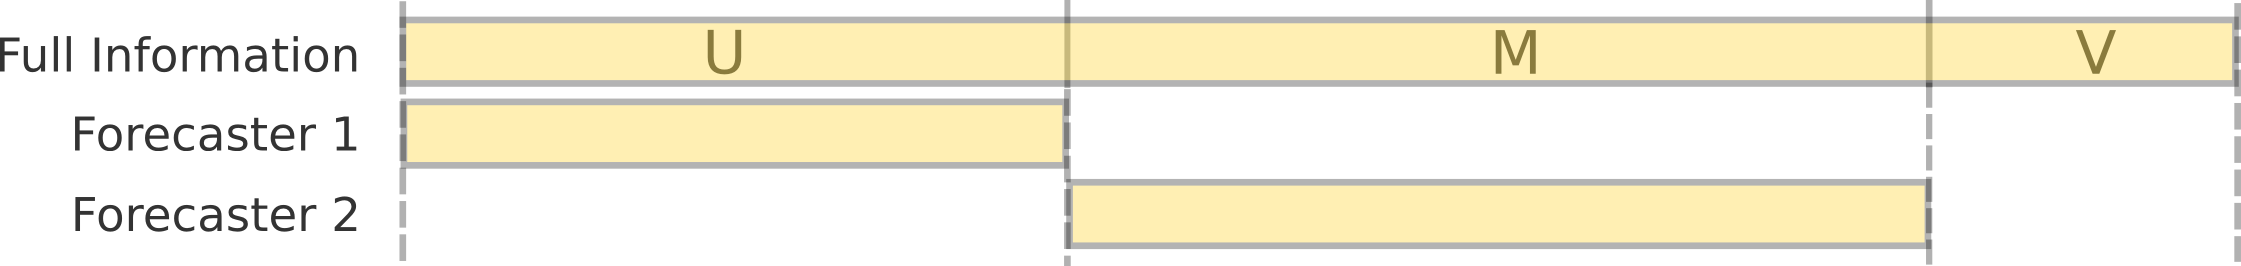
\includegraphics[width = \textwidth]{N=2.png} % requires the graphicx package
  \caption{Illustration of Information Distribution among Two Forecasters.
%   The top bar represents all possible information that can be known about $Y$. The bar leveled horizontally with Forecaster $j$ represents the $j$th forecaster's information set.
   }
     \label{InfoStr}
   \vspace{-0.5em}
\end{figure}

%In particular,  any variation in the forecasts is assumed to stem from information available to the forecasters and how they decide to use it. 
% Such diversity forms the basis of a novel modeling framework known as the \textit{partial information framework}.

% The result is a fundamentally different, yet extremely broadly applicable modeling framework, called the \textit{partial information framework}.
% This resulted in two publications that consider different prediction setups and propose model-based aggregators that extremize the average of the forecasters' log-odds  \citep{satopaa, satopaa2014probability}.
% This strictly empirical discovery was the initial reason that led me to collaborate with the GJP. The first two papers consider different prediction setups and propose model-based aggregators that extremized the forecasters' average log-odds  \citep{satopaa, satopaa2014probability}.
%%The first paper constructs a model-based aggregator that extremizes the average of the forecasters' log-odds \citep{satopaa}. The second paper considers a time-series context in which the forecasters are allowed to update their predictions whenever they felt the likelihood of the target event had changed \citep{satopaa2014probability}. The proposed aggregator is based on a dynamic linear model that extremizes the forecasters' average log-odds.  
%Even though these aggregators outperform other techniques in practice, they fail to explain the cause of the bias that extremization aims to correct. This bias turns out to be fundamentally linked with the 

% \vspace{-0.2em} \subsection{Partial Information Framework} \vspace{-0.2em}
 \vspace{0.5em}
\noindent
\textbf{2.1. PARTIAL INFORMATION FRAMEWORK:}
% Forecast aggregation literature by and large agrees that the goal is to collect and combine  information from different forecasters (see, e.g., \citealt{armstrong2})
%% (see, e.g., \citealt{forlines2012heuristics, armstrong2, dawid1995coherent})
%In fact, \cite{satopaamodeling} provide simple examples showing that optimal aggregation is not well-defined without assumptions on the information structure among the forecasters. To illustrate, consider two forecasters whose information sets are shown in Figure \ref{InfoStr}. In this diagram full information is represented by the unit interval. Forecaster 1 knows $U \cup M$ while forecaster 2 knows $M \cup V$. Ideally, an aggregator would utilize the forecasters' combined information, namely $U \cup M \cup V$.
%%Therefore nobody knows information in $W$. 
%Unfortunately, averaging aggregators do not behave like information aggregators. Instead, they assume that all forecasters use the same information and hence never appear more informed than the most informed individual forecaster \citep{satopaa2015combining}. This dramatically under-estimates the amount of combined information and leads to an under confident aggregate.  On the other hand, by assuming partially overlapping information sets, the partial information framework is able to estimate an aggregate that reflects the forecasters'  combined information.
%To make this specific, 
Consider $N$ forecasters and suppose forecaster $j$ predicts $X_j$ for some quantity of interest $Y$. The partial information framework assumes that $Y$ and $X_j$ are measurable random variables under some probability space $(\Omega, \F , \P)$. 
The $\sigma$-field $\F$ holds all possible information about $Y$. 
%Under the partial information framework, the forecasters operate under the same probability model but use different subsets of the full information. In fact, i
%In any Bayesian setup, with quadratic loss or some other loss function minimized by the conditional expectation, it is more or less tautological that
%More specifically,
%The 
Forecaster $j$ then predicts $X_j = \E(Y \| \F_j)$, where $\F_j \subseteq \F$ holds all information used in the forecast. In other words,  if the forecaster uses a simple rule, $\F_j$ may not be the full $\sigma$-field of information available to the forecaster but rather a smaller $\sigma$-field corresponding to the information actually used by the rule. Therefore $\F_i \neq \F_j$ if $X_i \neq X_j$, and forecast heterogeneity stems purely from information diversity.  
% Note, however, that if forecaster $j$ uses a simple rule, $\F_j$ may not be the full $\sigma$-field of information available to the forecaster but rather a smaller $\sigma$-field corresponding to the information used by the rule. Furthermore, if two forecasters have access to the same $\sigma$-field, they may decide to use different sub-$\sigma$-fields, leading to different predictions. 
%%%This is reminiscent of a forecasting algorithm that only uses
%%%a similarly restricted subset of information. 
%Therefore,
%information diversity does not only arise from differences in the available information, but also from how the forecasters decide to use it. 
%%\cite{satopaamodeling} provide simple examples to show
%%that the optimal aggregate is not well defined without
%%assumptions on the information structure among the forecasters.
%The covariance structure (\ref{cov_str}) provides leverage for regressing $Y$ on the $X_j$'s without a separate training set of past predictions and known outcomes. The resulting estimator,
%The main objective of the framework is to aggregate the forecasters' information into a consensus prediction. 
In practice, however, all details of the forecasters' information are not available to the aggregator. Instead, the forecasters typically reflect their information only through the predictions. Therefore the relevant aggregator under each specific instance of the framework is the \textit{revealed aggregator} $X'' := \E (Y \|
\F'')$, where $\F'' := \sigma(X_1, \dots, X_N)$ is the $\sigma$-field generated (or revealed) by the
$X_j$'s. 
% If $\E(Y^2) < \infty$, then among all variables measurable with respect to $\F''$, the revealed aggregator minimizes the expected quadratic loss and therefore provides a reasonable upper bound on aggregation efficiency. \cite{satopaa2015combining} show that $X''$ never reduces to a non-trivial weighted average of the forecasts, suggesting that information diversity, as a source of forecast heterogeneity, is fundamentally different from measurement error. 


%
%The framework introduces two
%%The partial information framework distinguishes
% benchmarks for aggregation efficiency. 
%% They differ in the degree to which they 
%The first is the {\em oracular} aggregator
%$X' := \E (\one_A \| \F')$, where $\F' = \sigma \left(\F_1, \dots, \F_N\right)$ represents all the information used by the forecasters. Given that aggregation cannot be improved beyond using all the information  of the forecasters, the oracular aggregator represents a theoretical optimum and is therefore a reasonable upper bound on estimation efficiency. 
%%Note that if a forecaster chooses to discard
%%some of the available information, then, for the purposes of aggregation,
%%that information may as well not exist. 
%In practice, however, information comes to the
%aggregator only through the forecasts $\{X_j : j = 1, \dots, N\}$. Given that $\F'$ generally cannot be constructed from these forecasts alone, no practically feasible aggregator can be expected to perform as well as $X'$.  Therefore, a more achievable benchmark is the \textit{revealed} aggregator $X'' := \E (\one_A \|
%\F'')$, where $\F'' = \sigma \left(\sigma(X_1), \dots, \sigma(X_N)\right)$ is the $\sigma$-field generated (or revealed) by the forecasts. If $\E(Y^2) < \infty$, then among all variables measurable with respect to $\F''$, the revealed aggregator minimizes the expected quadratic loss and is therefore considered the relevant aggregator under each specific instance of the framework. 

%
%Even though the partial information framework, as specified
%        above, is too theoretical for direct application, it highlights
%        the crucial components of information aggregation and hence
%        facilitates formulation of more specific models within the
%        framework.  One particularly close specification is called the
%        \textit{Gaussian partial information model}. This model introduces $N+1$ auxiliary variables, called the \textit{information variables}, that follow a multivariate Gaussian distribution with a particular covariance pattern:
%\begin{align}
%\left(\begin{matrix} Z_0 \\ Z_{1}\\ \vdots \\ Z_{N} \end{matrix}\right) &\sim \mathcal{N}_{N+1}\left( 
%%\left(\begin{matrix} 
%%\mu_1 \\ \boldsymbol{\mu}_2
%% \end{matrix}\right) =
% \boldsymbol{0}, \left(\begin{matrix} 
%1 & \diag(\bSigma)'\\
%\diag(\bSigma) &\bSigma\\
% \end{matrix}\right) 
% :=
% \left(\begin{array}{c | c c cc }
%1 & \delta_1 & \delta_2 & \dots & \delta_N  \\ \hline
%\delta_1 & \delta_1 &\rho_{1,2} & \dots & \rho_{1,N}   \\ 
%\delta_2 & \rho_{2,1} & \delta_2 & \dots & \rho_{2,N}  \\ 
%\vdots & \vdots & \vdots & \ddots & \vdots  \\ 
%\delta_N & \rho_{N,1} & \rho_{N,2} & \dots & \delta_N\\ 
% \end{array}\right)\right).  \label{NExperts}
%\end{align}
%The target outcome is given by $Y = g(Z_0)$, where $g(\cdot)$ is an application-specific link function that fully specifies the model instance. In general it makes sense to have $g(\cdot)$ map from the real numbers to the support of $Y$. For instance, if $Y \in \{0,1\}$, then $g : \R \to \{0,1\}$. The fact that $\Var(Z_0) = 1$ is irrelevant because this choice can be compensated by the link function.
% 
%        
%        



%
%%For one, due to the inability of the forecasters to identify clearly the basis to their predictions, the details of the information sets can almost always be rendered unattainable.
%%The first and most important step is to separate out those details of the information set that matter for aggregation and can be estimated in practice. 
%%To guide estimation, 
%%The key to applying this framework in practice is to observe that 
%Under these assumptions the amount of information can be measured and understood in terms of variance \citep{satopaa2015partial}. In particular,
%%   under the above assumptions of the partial information framework,  
%%   a) more information leads to higher variance, and b) common information suggests higher covariance among the forecasters. More formally,
%$\Var(Y)$ represents the maximum amount of information that can be known about $Y$, $\Var(X_j)$ is the amount of information used by forecaster $j$, and
%%and $\Var(X_j)$ quantify the amount of information in $\F$ and $\F_j$, respectively.  
%%represents the total amount of information and $\Var(X_j)$ is the amount of information used by forecaster $j$. 
% $\Cov (X_{i} , X_{j})$ can be interpreted as the amount of information overlap between forecasters $i$ and $j$. For example, in Figure \ref{InfoStr},
% \begin{align*}
% \Var(Y) &= 1.0, &&& \Var(X_1) = |U \cup M| &= 0.6,\\
% \Var(X_2) = |M \cup V| &= 0.5, &&& \Cov(X_1, X_2) = |M| &= 0.25.
% \end{align*}
%%Therefore increased variance suggests more information and is generally deemed helpful. This stands in clear contrast with standard statistical models that often regard higher variance as increased noise. 
%To illustrate why this works, consider a group of forecasters making probability estimates for a binary event. Forecasters with no or very little information are likely to report probabilities close to $0.5$, a.k.a., the non-informative estimate. On the other hand, highly informed forecasters are more likely to make predictions closer to the extremes at zero and one. Therefore more information leads to higher variance in the predictions. If two forecasters have high information overlap, they tend to report similar predictions and hence present higher covariance. The forecasters' information structure is therefore
%%The sizes of all such pairwise overlaps and individual sets of information are
% summarized by their covariance matrix $\bSigma_X :=  \Cov\left((X_1, \dots, X_N)'\right)$.
%%  For this reason covariance matrix estimation is central challenge in the applications of the partial information framework. 
%% Furthermore, 
% By interpreting $Y$ as a forecast based on full information, $\bSigma_X$ can be extended to the covariance of all model variables as follows:
%%, and common information suggests higher covariance among the forecasters. 
%%If $\X = (X_1, \dots, X_N)'$ collects all forecasts, the covariance matrix of the model variables $Y, X_1, \dots, X_N$ summarizes the distribution of information in the problem and must respect the following pattern:
%% In particular, \cite{satopaa2015partial} 
%%explain that in practice variance can be used to quantify information and
%% Fortunately, it is possible to deduce the amount of information used by a forecaster.  \cite{satopaa2015partial} 
%% show that, without any further assumptions, the covariance matrix $\bSigma_X$ of the $X_j$'s extends to the unknown $Y$ as follows:
%\begin{align}
%\bSigma := \Cov\left((Y, X_1, \dots, X_N)'\right) &=  \left( \begin{matrix} 
% \Var(Y)  & \diag(\bSigma_X)'  \\
%\diag(\bSigma_X) & \bSigma_X \\
%\end{matrix} \right), \label{cov_str}
%\end{align}
%where 
%%$\bSigma_X = \Cov(\X)$ and
%$\diag(\bSigma_X)$ denotes the diagonal of $\bSigma_X$. 
%%This describes the covariance structure of all model variables. 
%%The fact that $\bSigma$ must be positive semidefinite places a constraint on $\bSigma_X$. 
%%In particular, the matrix $\bSigma$ is positive semi-definite if and only if
%% Intuitively, 
%%for any given $X_1, \dots, X_N$, the corresponding $\bSigma$ satisfies $h(\bSigma) \in \mathcal{S}_{+}^{N+1}$ if there exists some random variable $Y$ such that all $X_1, \dots, X_N$ are conditionally unbiased for $Y$. In other words, $X_1, \dots, X_N$ must be jointly conditionally unbiased for some $Y$. 
%%Intuitively, $\bSigma_X$ satisfies this constraint if all the forecasts $X_j$ are simultaneously consistent with (possibly different) sets of information about some common yet unknown $Y$. \cite{satopaa2015partial} discuss  covariance matrix estimation under this constraint. 
%%, then the corresponding $\bSigma$ satisfies $h(\bSigma) \in \mathcal{S}_{+}^{N+1}$. 
%Given that $\bSigma$ must be positive semidefinite,  (\ref{cov_str}) places a  partial information specific constraint on $\bSigma_X$. In particular,  \cite{satopaa2015partial} explain that $\bSigma_X$ satisfies this constraint if and only if all the forecasts $X_j$ are simultaneously consistent with (possibly different) sets of information about some common yet unknown $Y$. 
%% \cite{satopaa2015partial} explain how the fact that $\bSigma$ must be positive semidefinite places a constraint on $\bSigma_X$.
%


%\marginpar{this is not correct; the constraint is on sigmaX, there must exist some Y such that blaah blaah}


% This covariance matrix summarizes information among the forecasters. In particular, $\Var(Y)$ is the maximum amount of information that can be known about $Y$, $\Var(X_j)$ is the amount of information used by forecaster $j$, and 
%%and $\Var(X_j)$ quantify the amount of information in $\F$ and $\F_j$, respectively.  
%%represents the total amount of information and $\Var(X_j)$ is the amount of information used by forecaster $j$. 
% $\Cov (X_{i} , X_{j})$ can be interpreted as the amount of information overlap between forecasters $i$ and $j$.  For example, in Figure \ref{InfoStr},
% \begin{align*}
% \Var(Y) &= 1.0, &&& \Var(X_1) = |U \cup M| &= 0.6,\\
% \Var(X_2) = |M \cup V| &= 0.4, &&& \Cov(X_1, X_2) = |M| &= 0.15.
% \end{align*}
% Therefore increased variance suggests more information and is generally deemed helpful. This stands in clear contrast with standard statistical models that often regard higher variance as increased noise. 
%  Why does this work? Consider a forecaster making a probability estimate.  First, note that a fully informed forecaster predicts  $X_j = Y$ while a forecaster with no information predicts the prior mean $X_j = \E(Y) = \E(Y|\F_0)$, where $\F_0 = \{\emptyset, \Omega\}$ is the trivial $\sigma$-field. Therefore as the forecaster becomes more informed, $\F_j$ grows from $\F_0$ to $\F$ and, consequently, $\Var(X_j)$ increases from $0$ to $\Var(Y)$. Second, two forecasters with high information overlap are likely to report very similar predictions and hence present higher covariance.

%% SPECIFICATION 

%At this level of specificity, the model, while too general to be applied, is almost certainly correct.

Even though the partial information framework, as briefly described above, is intuitively appealing, it is clearly too abstract to be applied in practice. Therefore, if it is to ever become common practice in forecast aggregation, a close yet practical specification within the framework must be introduced and made accessible to practitioners. Fortunately,  \cite{satopaa2015partial} explain that this only requires one additional assumption, namely the choice of a parametric family for the joint distribution of $Y, X_1, \dots, X_N$. 
%Different choices lead to different partial information models. 
% In order to construct a more specific model within the framework, a joint distribution for the model variables $Y, X_1, \dots, X_N$ must be specified.
 They provide both intuitive and technical motivations for using the multivariate Gaussian distribution
%  The resulting model, named the \textit{Gaussian partial information model}, has been extremely successful. 
%  First, \cite{satopaamodeling} use it to provide intuition on when and how much the average forecast should be extremized. Second, \cite{satopaa2015partial} estimate $\bSigma_X$ for forecasters addressing more than one related problems and
%  
and apply the resulting \textit{Gaussian partial information model} to real-world prediction polls, involving both probability and real-valued forecasts. In both cases, 
%the model is extremely successful. In particular, 
the revealed aggregator achieves large performance improvements over the common measurement-error-based aggregators, suggesting that  information diversity is the more important  source of forecast heterogeneity. 


%\marginpar{Metnion how different this is: variance etc.}

%Intuitively, this choice can be motivated by a pool of $M$ information particles. Each particle, which can be interpreted as representing a piece of information, has either a positive or negative effect on $Y$. The total sum (integral) of these particles determines the final value of $Y$. Each forecaster, however, observes only the sum of some subset of the particles. Based on this sum, the forecaster makes an estimate of $Y$. 
%If
%the particles are independent
%and have small tails, then as $M \to \infty$, the joint distribution
%of the forecasters' observations will be asymptotically
%Gaussian.  Therefore, given that the number of such particles in a real-world setup is likely to be large, it makes sense
%to model the forecasters' observations as jointly Gaussian.

%In many applications, however, $Y$ and $X_j$ may not be supported on the whole real line. For instance, in probability forecasting of binary events typically  $Y \in \{0,1\}$ and $X_j \in [0,1]$. Fortunately, this limitation can be easily handled by borrowing from the theory of generalized linear models \citep{mccullagh1989generalized} and utilizing a \textit{link function}. The following \textit{Gaussian model} makes this concrete by introducing $N+1$ auxiliary variables, called the \textit{information variables}, that follow a multivariate Gaussian distribution with the covariance pattern (\ref{cov_str}):
%\begin{align}
%\left(\begin{matrix} Z_0 \\ Z_{1}\\ \vdots \\ Z_{N} \end{matrix}\right) &\sim \mathcal{N}_{N+1}\left( 
% \boldsymbol{0}, \left(\begin{matrix} 
%1 & \diag(\bSigma)'\\
%\diag(\bSigma) &\bSigma\\
% \end{matrix}\right) 
% :=
% \left(\begin{array}{c | c c cc }
%1 & \delta_1 & \delta_2 & \dots & \delta_N  \\ \hline
%\delta_1 & \delta_1 &\rho_{1,2} & \dots & \rho_{1,N}   \\ 
%\delta_2 & \rho_{2,1} & \delta_2 & \dots & \rho_{2,N}  \\ 
%\vdots & \vdots & \vdots & \ddots & \vdots  \\ 
%\delta_N & \rho_{N,1} & \rho_{N,2} & \dots & \delta_N\\ 
% \end{array}\right)\right).  \label{NExperts}
%\end{align}
%The target outcome is given by $Y = g(Z_0)$, where $g(\cdot)$ is an application-specific link function that fully specifies the model instance.


%Abstract first then explain that must be made practical yet close. Show details!
%Must make clear that this is very broadly applicable. 
%Fundamentally different: never reduces to, say, convex combo.



% \vspace{-0.2em} \subsection{Future Research}  \vspace{-0.2em}
 \vspace{0.5em}
\noindent
\textbf{2.2. CURRENT AND FUTURE RESEARCH:}
This work proposes an alternative to a core statistical concept, namely measurement error, and
%Given that measurement error is one of the core concepts in statistics, an enormous amount of research derives from it. Information diversity is a natural yet fundamentally different alternative to it.
 leads to a new modeling paradigm that is fundamentally different
% yet in many applications more appropriate than
from classical statistics. 
% hence 
%Given the fundamental nature of this innovation, the partial information framework
This suggests a range of theoretical and applied projects in statistics and other related fields. 
% much future research, involving both theoretical and applied projects. 
 The following illustrates some specific projects:

% \vspace{0.5em}
%\noindent
%a)  \cite{satopaa2015partial} apply the Gaussian model in a setup where the forecasters participate in separate yet similar prediction problems or give repeated forecasts on a single recurring event. In the most extreme case, however, only a set of forecasts of a single unknown outcome are available. How should the forecasts be aggregated in such a low-data setting?
%% \cite{satopaa2015combining} suggest that any type of weighted average (or some other measure of central tendency) is a poor choice. 
%%A better alternative was discussed by \cite{satopaamodeling}. They assume that $\bSigma_X$ is compound symmetric and then combine the forecasts with the revealed aggregator under the corresponding Gaussian partial information model. 
% Developing a partial information aggregator that can be directly applied to a single set of forecasts is certainly a future research direction with potential for high impact. One idea is to first derive the aggregator based on the Gaussian model and then integrate out any unknown parameters with respect to their posterior distribution. Currently, we have
%work in progress analyzing such \textit{Bayes-Gaussian aggregators} but much more work is needed \citep{ernst2015, satopaaBayesGaussian}. 
%
%
% \vspace{0.5em}
%\noindent
%b)  Most probability aggregation procedures use one probability estimate per forecaster, even though it is common for experts studying real problems to update their probability estimates over time. \cite{satopaa2014probability} advance into unexplored areas of probability aggregation by considering a dynamic context in which experts can update their beliefs at random intervals. Overall, this paper was very well received. The aggregator therein, however, is based on measurement error. Therefore, an interesting future project would be to utilize martingale theory and develop a time-series aggregator based on partial information. 
%
% \vspace{0.5em}
%\noindent
%c)  The partial information framework can be also applied to forecasts made by different models. This suggests many contributions in machine learning. For instance, semi-supervised learning refers to setups with a large amount of data of which only a relatively few have been labeled. Many of the commonly used ensemble techniques, such as stacking or Bayesian averaging, however, require labeled observations to combine the individual models' predictions. In the contrary, the partial information framework can aggregate predictions without labeled data. This suggests an opportunity for better aggregation and hence overall improved prediction accuracy.


\begin{enumerate}[i)]
\itemsep-0.3em 
\item
% \cite{satopaa2015partial} apply the Gaussian model in a setup where the forecasters participate in separate yet similar prediction problems. In the most extreme case, however, only a set of forecasts of a single unknown outcome are available. How should the forecasts be aggregated in such a low-data setting?
% \cite{satopaa2015combining} suggest that any type of weighted average (or some other measure of central tendency) is a poor choice. 
%A better alternative was discussed by \cite{satopaamodeling}. They assume that $\bSigma_X$ is compound symmetric and then combine the forecasts with the revealed aggregator under the corresponding Gaussian partial information model. 
 Developing a partial information aggregator for a set of forecasts of a single outcome is a future research direction with potential for high impact. One idea is to first derive the aggregator based on the Gaussian model and then integrate out any unknown parameters with respect to their posterior distribution. Currently, we have
work in progress analyzing such \textit{Bayes-Gaussian aggregators} but much more work is needed \citep{ernst2015, satopaaBayesGaussian}. 
 

 %The first step is to develop an aggregator that is both marginally consistent and expanding. Finding an aggregator that maintains forecasters' reliability seems more difficult. 

%\item A promising empirical direction is the Bayesian approach. These techniques have been found superior to the likelihood-based alternatives in many applications with small or moderately sized datasets. Therefore, given that the number of forecasts in a prediction poll is typically quite small, a Bayesian approach is likely to improve the quality of the final aggregate. This would involve  developing a prior distribution for $\bSigma_{X}$ -- a problem that seems interesting in itself because of the semidefinite constraints that  (\ref{cov_str}) places on $\bSigma_{X}$ \citep{satopaa2015partial}.  
\item Information diversity is not only relevant in estimation but also offers new directions in other areas of statistics. For instance, some of our current work explores information diversity in testing hypotheses about a binary outcome \citep{satopaaTesting}. The hope is to eventually extend this work to simultaneous testing of multiple informationally overlapping hypotheses.

\item Most aggregation procedures use one estimate per forecaster, even though it is common for experts to update their beliefs over time. 
%\cite{satopaa2014probability} advance into unexplored areas of probability aggregation by considering a dynamic context in which experts can update their beliefs at random intervals. Overall, this paper was very well received. The aggregator therein, however, is based on measurement error. Therefore, 
Therefore an interesting future project is to utilize martingale theory and develop a time-series aggregator based on partial information. 

\item Information diversity can be also applied to model predictions. This suggests many contributions in machine learning. For instance, semi-supervised learning refers to setups with a large amount of data of which only a relatively few have been labeled. While the commonly used ensemble techniques, such as stacking or Bayesian averaging, require labeled observations to combine the individual models' predictions, the partial information framework can aggregate predictions without labeled data. This suggests an opportunity for improved aggregation efficiency.
% and hence overall improved prediction accuracy.

\end{enumerate}

% \vspace{1em} \section{Public Reporting of Hospital Mortality Rates}   \vspace{-0.2em}
%\subsection*{}
%With a view to providing the public with information about the quality of hospitals, Medicare runs a website called �Hospital Compare� (http://www.medicare.gov/hospitalcompare/). Among other things, for each hospital, Hospital Compare provides information about the mortality rate of patients treated for a heart attack, or �acute myocardial infarction� (AMI). If you enter your zip code at the website, Hospital Compare will tell you about hospitals near where you live. Nationally, for a person who arrives at the hospital alive, the 30 day mortality rate following AMI is in the vicinity of 15\%. The website�s reported hospital-specific mortality rates are based on Medicare claims data and a random effects logit model in which hospitals enter as a random intercept and adjustments are made for risk factors describing individual patients, for instance age and prior heart attacks. The number reported by Hospital Compare is essentially an indirectly standardized mortality rate for each hospital, adjusting for measured risk factors describing the patient. An indirectly standardized rate is a constant multiple of a ratio of two predictions for the mortality of the patients actually treated at that hospital, namely, in the numerator, the model�s predicted mortality rate if these patients were treated at this hospital, and in the denominator, the model�s predicted mortality for the same patients if treated at a typical hospital. A ratio substantially above one is interpreted as �worse than average risk� and a ratio substantially below one is interpreted as �better than average risk�. The website describes most hospitals as ''no different than the national average.'' 
%
%Some small hospitals treat a few AMIs per year, whereas there is a hospital in New York that treats on average about two AMIs per day. Mortality rates from small hospitals are quite unstable, and the random intercepts model used by Hospital Compare shrinks these rates to resemble the National average. The model says: �if there is not much data about your hospital, then we predict that you are average.� For any one small hospital, there is not much data to contradict that prediction. So the model claims that the mortality rate at each small hospital is close to the National average. Is this a discovery or an assumption?
%
%If it is a discovery, then it is a surprising discovery. A fairly consistent finding in health services research is that, adjusting for patient risk factors, mortality rates are typically higher at low volume hospitals (Gandjour, Bannenberg, and Lauterbach 2003; Halm, Lee, and Chassin 2002; Luft, Hunt, and Maerki 1987; Shahian and Normand 2003). Indeed, this pattern is unambiguously evident in the data used to fit the Hospital Compare model. Therefore, sound general advice would be to avoid low volume hospitals for treatment of AMI.
%
%So, is the finding of average risk at small hospitals a discovery or an assumption? Actually, it is neither: it is a mistake. The model is not properly calibrated; see Dawid (1982) for discussion of calibration. Although there is very little data about any one small hospital, hence very little data to check a statement about one small hospital, there is plenty of data about small hospitals as a group. When you add up Hospital Compare�s predictions for all small hospitals, it is unambiguously clear that the risk at small hospitals as a group is well above the national average; see Silber et al. (2010).
%
%There is, here, a general principle. A Bayesian model can use all of the data to make an individualized prediction that is difficult to check as a single prediction. It is possible that this individualized prediction is better than relying upon general advice, because it is possible that this individualized prediction is tapping into distinctions evident in the data but not reflected in general advice. But if the general advice is correct as general advice, the individualized predictions should not aggregate to contradict correct general advice. For instance, if the risk at low-volume hospitals as a group is well above the national average, so general advice would direct you away from low-volume hospitals if you had a near-by alternative, then individualized predictions should not aggregate to contradict that general advice. If the data warrants this, the individualized predictions may identify particular low volume hospitals with average or better than average mortality, but checkable aggregates should agree. As a check on whether a Bayesian model is calibrated, checking individualized predictions against general advice has two virtues. First, what it checks can fail to hold, so it can reject some models as inadequate. Second, what it checks is relevant: the check is against the advice you would fall back upon if individualized predictions were unavailable. A model may be detectably false in an irrelevant way � it may use a double exponential distribution where a logistic distribution would have been better � but that model failure may have negligible consequences for its recommendations. However, if the model contradicts correct general advice, then there is reason to worry about its individualized predictions.
%

%Medicare's Hospital Compare is a patient-oriented website that 
%%provides information on how well hospitals provide recommended care to their patients. The site 
%is hosted by the U.S. Department of Health \& Human Services (HHS) with the goal of helping patients to make informed decisions about health care.
 \vspace{0.5em}
\noindent
\textbf{3. PUBLIC REPORTING OF HOSPITAL QUALITY:} 
Medicare's Hospital Compare is a website
%\footnote{Visit \url{http://www.medicare.gov/hospitalcompare} for more information}
 where patients can select multiple hospitals and compare their performance related to heart attack, pneumonia, and other conditions. For acute myocardial infarction (AMI) mortality in 2008, of 4,311 U.S. hospitals, the Hospital Compare model asserted that none were worse than average and nine were better than average. This is a very surprising result because some of these hospitals treat only a few AMI cases per year, while others treat several cases each week. The medical literature \citep{luft1987volume, gandjour2003threshold} has consistently indicated that after adjusting for patient risk factors, there is a higher risk of death at a low-volume hospital. Therefore, sound \textit{general advice} would
be to avoid low volume hospitals. Even though this relationship is clear in the data used by Hospital Compare, they fail to report any such pattern. 

This failure is due to Hospital Compare's efforts to stabilize the estimated mortality rates of low-volume hospitals by shrinking them towards the U.S. national average. During my doctoral studies I have collaborated closely with the Center for Outcomes Research at the Children's Hospital of Philadelphia to correct this shortcoming. 
Even though our work is about methodology, it aims to shift the policy paradigm for public reporting, to a more patient-centered, Bayesian perspective \citep{publicReporting, publicReporting2}.  More specifically, our models assume low-volume hospitals to be similar to other low-volume hospitals and hence stabilize their estimates by shrinking them towards the average of hospitals with similar volume and facilities.
%
% Hospital Compare, however, assumes no relationship between volume and mortality. 
%%This is an unreasonable assumption given that the literature suggest that mortality rates tend to be higher at low-volume hospitals (see, e.g., \cite{tu2001relationship, halm2002volume}). 
%It is important to note that Hospital Compare could have developed a model that allowed the empirical data to speak to the issue of whether a systematic volume-outcome relationship is present. Instead Hospital Compare employed an over-riding assumption that the true mortality rates are random and independent of any hospital-level characteristic. 
%
%In public reporting it is not enough to give just the single best estimate of the mortality rate at a given hospital. The uncertainty associated with this estimate must also be reported because  the patient has the right to know that the performance of a high-volume hospital is typically known with greater certainty than the performance of a low-volume hospital. Unfortunately, Hospital Compare's  over-stabilizing strategy underestimates the true level of uncertainty, and as a result, the Hospital Compare website presents
%%the performance of low-volume hospitals is estimated to be unrealistically good with unrealistically high certainty, and 
%low-volume hospitals as almost identical to the high-volume hospitals. 
%
%%Our work improves upon the Hospital Compare model by a) shrinking mortality rates slightly towards the average of hospitals with similar volume and facilities, and b) using Bayesian methodology that is ideally suited for comparing risks and evaluating any uncertainty in the resulting performance estimates. Reporting the degree of uncertainty in the performance estimates is very important because the patient has the right to know that the performance of a high-volume hospital is typically known with greater certainty than the performance of a low-volume hospital. Hospital Compare's over-stablizing shrinkage strategy, however, dramatically underestimates the inherent uncertainty in the performance of low-volume hospitals. As a result, the performance of low-volume hospitals is reported unrealistically low with unrealistically high certainty making them appear almost identical to the high-volume hospitals.
%equivalent or even higher certainty than the performance of high-volume hospitals. 
%Therefore Hospital Compare does not only estimate the low-volume hospitals to be better than what they really are, but also presents these incorrect results with unrealistically high confidence. 
%
%
%This year our work has focused on modeling AMI mortality rates. Our models improve upon Hospital Compare by shrinking mortality rates slightly towards the average of hospitals with similar volume and facilities. 
 The models form a hierarchy where each subsequent model is more flexible than the previous one and has the choice of reverting back to the Hospital Compare model if the empirical data finds this appropriate. 
%We have developed a hierarchy of models that build on top of the Hospital Compare model. Each subsequent model incorporates hospital volume and is more flexible than the previous one. It is important to note that all of our models have the choice of reverting back to the Hospital Compare model if the empirical data finds this appropriate.
 None, however, do so. Instead they find a clear volume-outcome relationship and no longer contradict general advice. 
%  where both performance and the accuracy to estimate it improve as volume increases. 
% the higher-volume hospitals having a lower mortality rate with higher estimation certainty. 
Our AMI mortality data, which are a very careful imitation of Medicare's data and consist of about 340,000 patients distributed across about 4,300 hospitals, support all of our models much more than the Hospital Compare model.
% In particular, our models no longer contradict general advice. 

%With this form of careful model development, strong empirical evidence, and 


%Furthermore, unlike the Hospital Compare model, our models are based on Bayesian statistics that is ideally suited for comparing risks and evaluating any uncertainty in the performance measures.

%im to shift the policy paradigm for public reporting in 

%While our models predict the mortality rate at low-volume hospitals (bottom 20\% in terms of volume) with good accuracy, the Hospital Compare model predicts the mortality rate to be around 22\% when it really is around 29\%. Therefore Hospital Compare drastically underestimates the death rate at low-volume hospitals and ends up giving advice that is both misleading and harmful for the patient. 
%
%It is evident that any model selected for public reporting will be faced with other competing alternatives. To decide whether a new model should be adopted, it will be necessary to develop a principled framework for model selection. Our goal is  to develop a \textit{predicted survival maximization approach} that uses the patients' characteristics (sex, age, zip-code, and Hospital Referral Region) and medical history (diabetes, hypertension, cancer, etc.) to 
%%patients' zip-codes and Hospital Referral Regions (HRR) 
%predict their survival at any near-by hospitals. Assuming that patients always choose the near-by hospital that maximizes their survival, we can estimate the overall rate of survival under any model. This selection procedure is very closely related to the patient's actual experience at Medicare's Hospital Compare website and therefore has a high priority in our work. Currently we have preliminary ideas on how to implement this approach, but more work is needed. 

%The models should also be compared with respect to \textit{calibration}, which measures how closely the frequency of deaths agrees with the assigned mortality rate. For instance, the actual rate of deaths is 10\% for all those patients for whom a well-calibrated model assessed the probability of dying to be 10\%. Given that our data consist mostly of surviving patients, the models have much more information about non-dying patients and hence tend to be very well-calibrated when predicting low death rates (below 30\%). Unfortunately, under such survival-dominated data, the models end up over-focusing on the surviving group (\citet{chen2009learning, wallace2012class}) and, as a result, give miscalibrated predictions at high death rates (above 70\%). Even though our models are overall more calibrated than the Hospital Compare model, future improvements are needed to assure better calibration at high death rates.


%
%Studying other hospital-level characteristics besides volume is also important. For instance, the CMS-Committee of the Presidents of the Statistical Societies (COPSS) Report (\cite{ash2012statistical}) repeatedly mentions the importance of distinguishing between rural and urban hospitals. See \cite{james2007myocardial} for evidence that patients with AMI have higher mortality rates in rural hospitals than in urban hospitals. Other interesting hospital-level characteristics are nurse-to-bed ratio, resident-to-bed ratio, hospital technology status, and teaching status. Our plan is to study which of these hospital-level characteristics have a systematic relationship with better performance and hence should be included in the model. Furthermore, we aim to model interactions between the hospital-level and patient-level characteristics to gain insight on which types of hospitals are better at treating each type of patients. 


%This gives us our third and final hypothesis:
%\begin{quote}
%\textbf{Hypothesis 3:}  Letting the hospitals-specific effects on mortality to depend on more than one hospital-level characteristic will improve the accuracy of our model and also provide insight on which hospital-level characteristics have a systematic relationship with better performance.
%\end{quote}



%This leads to our first hypothesis:
%\begin{quote}
%\textbf{Hypothesis 1:} The results for Pneumonia and Congestive Heart Failure will be qualitatively similar to the results on AMI mortality rates.
%\end{quote}


%In our first paper, which is currently being  prepared, our models are shown to be much more likely given the data and give

%also to capture the true nature of previously unseen low-volume hospitals much better than the Hospital Compare model. 
%our models are shown to be superior to the Hospital Compare model based on 
%In addition to having constructed a more accurate and informative model for the mortality rates, I have detected a simple, yet powerful model comparison framework that makes use of the well-known Bayes factors. 

%All the necessary results have been computed and analyzed for 
%As the model is allowed increasing flexibility, the 

%The resulting predictions for the low-volume hospitals made by the Hospital Compare model and our more flexible models are strikingly different. 

%Much work remains to be done in model development for public reporting. 
%In the technical part of our work the goal is to eliminate three main limitations of our current models: First, all the models assume a unimodal and symmetric Gaussian distribution for the hospital-specific effects. It is unlikely that this is a realistic modeling assumption.
%%This assumption is rather unrealistic and results into low-volume hospitals that simultaneously have a high likelihood of being much better and much worse than any high-volume hospital. Such an uninformative statement is not very useful in decision making. The model is simply too constrained to encompass a low-volume hospital that is either clearly worse or clearly better than any high-volume hospital. 
%Second, all the models stabilize performance estimates by shrinking them towards a single point that may or may not depend on volume. Given that there are likely to be differently performing groups of hospitals at different levels of volume, each performance measure should be shrank towards the average of its associated group -- not the overall average of hospitals with the same volume. Third, fitting the models using the standard sampling-based approaches is computationally very demanding and can take weeks to complete. 
%%A typical criticism on the use of multiple shrinkage points revolves around the need to specify the number of groups before fitting the model. This specification is a subjective exercise and can lead to unrealistic results. 
%A solution to the first two limitations is to use non-parametric Bayesian methods (\cite{gelfand2005bayesian}) that rely heavily on the data to decide the number of groups and the overall shape of the distribution of the hospital-specific effects.  To address the third limitation, our goal is to develop optimization-based approaches (\cite{blei2006variational, nott2012variational}) that have the advantage of being very suitable for large datasets, having fast and guaranteed convergence to a locally optimal solution, and conveniently producing a model selection criterion as a side-effect.


%
%The key output of our model is an estimated \textit{posterior distribution} of the mortality rate at a given hospital. This is a statistical quantity that can be difficult to understand by patients who are not familiar with the statistics literature. For this reason, we are using  web-based questionnaires (MTurk) and experiments at the Wharton Behavioral Lab to detect a presentation format that is less likely to be misinterpreted and, hence, less likely to lead to incorrect hospital selection. The final product of our research will be a new publicly available website that presents accurate performance measures in a user-friendly format. The website will enable patients to type in their personal information (age, sex, and any medical history) and compare performance estimates that are personalized and hence more relevant to them. 


%% \vspace{-1em} \subsection{Future Research} \vspace{-0.2em}
% \vspace{0.5em}
%\noindent
%\textbf{3.1. FUTURE RESEARCH:} The largely unprincipled modeling practice in public reporting offers many research opportunities. 
%%For instance, we have found serious shortcomings in the models used for ranking liver transplantation centers.  
%Even though our work corrects some of the common misconceptions and lays down foundations upon which more principled public reporting can be developed, much work remains to be done.
%Our future work involves
In the future we plan to 
%to repeat our study of AMI on heart failure and pneumonia, for which we already have close imitations of Medicare's data. 
%have data that closely imitate that of Medicare's. 
% In particular, 
%The following enumeration provides some future direction. 
%\begin{enumerate}[i)]
%\item 
%Another interesting avenue is 
study models that allow hospital and patient characteristics to interact. Such
models would help us identify types of patients that each hospital treats particularly well
%For instance, 
%Second, our current models mostly separate patient and hospital characteristics. However, 
%letting the slope coefficients of the patient characteristics to change, say, linearly in the hospital characteristics, 
%Such a model would
% indicate for each hospital the type of patients it treats particularly well  
% what kind of hospitals are good at treating what kind of patients
  and
   also form the basis of a new publicly available website where patients can type in their personal information and compare performance estimates that are personalized and hence more relevant to them. 




%\item Unfortunately, the Hospital Compare model has become the ``gold standard'' in many areas of public reporting.
%%This means that models of many other conditions, such as pneumonia and heart failure, must be re-evaluated. 
%For instance, similar modeling mistakes have been made in rankings of liver transplantation centers. The nature of liver transplantation also poses additional questions: How well are the centers matching their available livers to patients? What is their mortality rate after controlling for the quality of these livers? To the best of our knowledge, no previous research has attempted to answer these specific questions. 

%
%Therefore many other areas such as 
% Pneumonia and Heart Failure. This along with other results and analyses is included in our first paper that is currently being prepared. Part of our future work is to replicate the analysis for pneumonia and congestive heart failure, and also extend our analysis to readmission rates. It is still unclear whether the results will be qualitatively similar to our results on AMI.
%\item Liver transplant
%\item Non-parametric models. All the models assume a unimodal and symmetric Gaussian distribution for the hospital-specific effects. It is unlikely that this is a realistic modeling assumption.
%\end{enumerate}

 \vspace{0.5em}
\noindent
%\section{Conclusion: Other Research Directions} 
\textbf{4. CONCLUSION AND OTHER RESEARCH DIRECTIONS: }
My research interests are not limited to these two projects, but also span many other areas. For one,
%I believe data collection in judgmental forecasting can be greatly improved by interactive elicitation of judgements.
%Also,
 given my background in computer science, I am broadly interested
in machine learning, computational statistics, and, in particular, the many scalability issues that classical statistical procedures
are facing in today�s �big data� boom. All in all, however, I enjoy working with subject-matter experts, always
look forward to forming new collaborations, and consider dirty real-world data not as a hindrance
to my research but rather as an opportunity to learn and develop new methodologies.




%\marginpar{Generally interesting in forecasting. and always looking for new collaborations. insights in forecasting. active sampling to boost predictive performance. }

%\bibliographystyle{myplain.bst}
\bibliographystyle{myapalike.bst}

%\def\FormatName#1{%
%  \def\myname{{Satop\"a\"a}, V.}%
%%  \def\myname{Silber, J. H.}%
%%  \def\myname{Ungar, L.}%
%  \edef\name{#1}%
%  \ifx\name\myname
%    \textbf{#1}%
%  \else
%    #1%
%  \fi
%}

\def\FormatName#1{%
  \IfSubStr{#1}{Satop}{\textbf{#1}}{#1}%
}


\bibliography{biblio}		% expects file "myrefs.bib"




\end{document}